\subsection{Method Comparison}

\begin{frame}{Comparison of Methods}
\begin{itemize}
\item 10 training frequencies logarithmically spaced between $10^{-3}$ and $10^4$\\
\item Tolerance of $10^{-12}$ for cutting off SVD's
in both methods\\
\bigskip
\item Size of ROMs: \\
\begin{itemize}
    \item Loewner Framework - 5 by 5
    \item Projection - 10 by 10
\end{itemize}
\end{itemize}

\centering
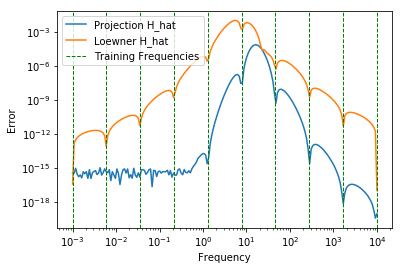
\includegraphics[width=7.5cm, height= 6cm]{comparison0.png}

\end{frame}
%%%%%%%%%%%%%%%%%%%%%%%%%%%%%%%%%%%%%%%%%%%%%%%%
\begin{frame}{Comparison of Methods}
\begin{itemize}
    \item Covert both ROMs to real domain\\
    \bigskip
    \item Size of ROMs: \\
    \begin{itemize}
        \item Loewner Framework - 8 by 8
        \item Projection - 15 by 15
    \end{itemize}
\end{itemize}

\centering
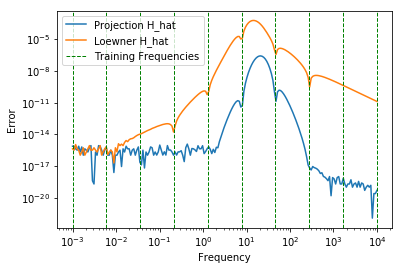
\includegraphics[width=7.5cm, height= 6cm]{comparison1.png}
\end{frame}
%%%%%%%%%%%%%%%%%%%%%%%%%%%%%%%%%%%%%%%%%%%

\begin{frame}{Comparison of Methods}
Compare ROM methods to the FOM in the time domain:\\
\bigskip
\begin{center}
 Let $u(t) = sin(2 \pi t)$, for $0 \leq t \leq 0.5$   
\end{center}

\centering
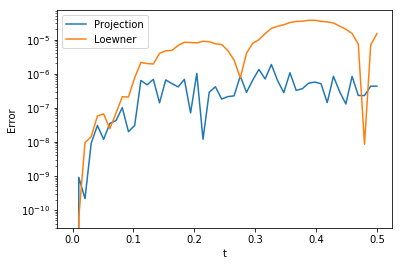
\includegraphics[width=7.5cm, height= 6cm]{comparison2.png}
\end{frame}
